\documentclass[10pt,a4paper]{article}
\usepackage[english]{babel}
\usepackage[utf8]{inputenc}
\usepackage[T1]{fontenc}
\usepackage{indentfirst}
\usepackage{anysize}
\marginsize{2.5cm}{1.8cm}{1.5cm}{1.7cm}

% Mathematical packages
\usepackage{amssymb,amsfonts,amsmath,amsthm}

% Table packages
\usepackage{multicol,multirow}

% Graphics packages
\usepackage{graphicx}
\usepackage[labelfont=bf]{caption}
\usepackage{subcaption}
\usepackage{tikz}
\usetikzlibrary{shapes,arrows,positioning,calc,fit,decorations.pathreplacing}

% Hyperlinks
\usepackage{hyperref}
\hypersetup{
    colorlinks=true,
    linkcolor=blue,
    filecolor=magenta,      
    urlcolor=cyan,
    pdftitle={Distributed Array Library},
    pdfpagemode=FullScreen,
}

% Algorithms
\usepackage{algorithm}
\usepackage{algpseudocode}

% Code listings
\usepackage{listings}
\usepackage{xcolor}
\definecolor{codegreen}{rgb}{0,0.6,0}
\definecolor{codegray}{rgb}{0.5,0.5,0.5}
\definecolor{codepurple}{rgb}{0.58,0,0.82}
\definecolor{backcolour}{rgb}{0.95,0.95,0.92}

\lstdefinestyle{mystyle}{
    backgroundcolor=\color{backcolour},
    commentstyle=\color{codegreen},
    keywordstyle=\color{magenta},
    numberstyle=\tiny\color{codegray},
    stringstyle=\color{codepurple},
    basicstyle=\ttfamily\footnotesize,
    breakatwhitespace=false,
    breaklines=true,
    captionpos=b,
    keepspaces=true,
    numbers=left,
    numbersep=5pt,
    showspaces=false,
    showstringspaces=false,
    showtabs=false,
    tabsize=2
}
\lstset{style=mystyle}

% TikZ styles
\tikzset{
    master/.style={draw, rectangle, fill=blue!20, minimum width=3cm, minimum height=1.5cm, text centered, rounded corners},
    worker/.style={draw, rectangle, fill=green!20, minimum width=2.5cm, minimum height=1.2cm, text centered, rounded corners},
    client/.style={draw, rectangle, fill=orange!20, minimum width=2.5cm, minimum height=1.2cm, text centered, rounded corners},
    arrow/.style={->, >=stealth, thick},
    data/.style={draw, rectangle, fill=yellow!10, minimum width=2cm, minimum height=0.8cm, text centered},
    socket/.style={<->, >=stealth, thick, red},
    replica/.style={draw, rectangle, fill=yellow!5, minimum width=2cm, minimum height=0.8cm, text centered, dashed}
}

% Table of contents configuration
\usepackage{tocloft}
\renewcommand{\cftsecleader}{\cftdotfill{\cftdotsep}}
\renewcommand*\contentsname{Table of Contents}
\renewcommand{\thepage}{\arabic{page}}

% Theorems and definitions
\theoremstyle{definition}
\newtheorem{definition}{Definition}[section]
\theoremstyle{remark}
\newtheorem*{remark}{Remark}

% Footnote configuration
\renewcommand{\thefootnote}{\fnsymbol{footnote}}

\begin{document}

% Title page
\title{Distributed Array Library with Fault Tolerance}
\author{
    \begin{minipage}[t]{0.3\textwidth}
        \centering
        \textbf{Student:}\\[5pt]
        {\large Arbués Pérez V.}\\
        National University of Engineering\\
        Faculty of Sciences\\
        e-mail: arbues.perez@uni.pe
    \end{minipage}
    \hfill
    \begin{minipage}[t]{0.3\textwidth}
        \centering
        \textbf{Student:}\\[5pt]
        {\large Sergio Pezo J.}\\
        National University of Engineering\\
        Faculty of Sciences\\
        e-mail: sergio.pezo@uni.pe
    \end{minipage}
    \hfill
    \begin{minipage}[t]{0.3\textwidth}
        \centering
        \textbf{Student:}\\[5pt]
        {\large André Pacheco T.}\\
        National University of Engineering\\
        Faculty of Sciences\\
        e-mail: andre.pacheco@uni.pe
    \end{minipage}
}
\date{\today}
\maketitle

% Abstract
\begin{abstract}
\hspace*{0.5cm}
This document presents the design, development, and implementation of a distributed library for processing large numerical arrays. The system is built upon a master-worker architecture and is implemented in both Java and Python, utilizing only native TCP sockets for inter-process communication, without relying on external messaging frameworks. Key features include automatic data segmentation, parallel processing of mathematical operations on worker nodes, and a robust fault tolerance mechanism based on heartbeats, data replication, and automatic replica promotion. The project also demonstrates interoperability between components written in different languages, showcasing the flexibility of a well-defined, language-agnostic communication protocol.

\vspace{5pt}
\textbf{Keywords:} Distributed Systems, Fault Tolerance, TCP Sockets, Parallel Processing, Data Replication, Interoperability.
\end{abstract}

\newpage
\tableofcontents
\newpage

% General introduction
\section{General Introduction}

Distributed systems are fundamental to modern computing, providing the scalability and resilience required to handle large-scale data processing tasks. This project focuses on the core principles of distributed systems by building a library from the ground up for managing and processing large numerical arrays across multiple nodes. The primary goal is to create a system that is both high-performing and fault-tolerant, using fundamental technologies rather than high-level frameworks.

The developed system implements a master-worker architecture where a central master node coordinates a cluster of worker nodes. Large arrays provided by a client are automatically segmented and distributed among the workers. Each worker then leverages multi-core processors to perform parallel computations on its assigned data segment. This approach allows for horizontal scalability, where adding more worker nodes directly increases the system's processing capacity.

A key aspect of this project is the implementation of a robust fault tolerance system. Using a heartbeat mechanism, the master node monitors the health of each worker. If a worker fails, the system automatically promotes a replica of the lost data on another worker, ensuring no data loss and maintaining service continuity. The entire project is implemented in both Java and Python to demonstrate that the principles and the communication protocol are language-agnostic, even allowing for a mixed-language cluster.

\section{Objectives}

\subsection{General Objective}
To design and develop a robust, scalable, and fault-tolerant distributed library for processing large numerical arrays, using fundamental distributed computing concepts and native TCP socket communication.

\subsection{Specific Objectives}
\begin{itemize}
    \item Implement a master-worker architecture capable of managing a cluster of processing nodes.
    \item Develop the complete system in two separate, language-specific implementations (Java and Python) to ensure protocol integrity.
    \item Design and implement a custom, JSON-based communication protocol over native TCP sockets.
    \item Implement automatic data segmentation and distribution of large arrays from a client to the worker nodes.
    \item Utilize multi-threading on worker nodes to achieve parallel processing of data segments.
    \item Implement a fault tolerance mechanism with heartbeat-based failure detection, data replication, and automatic replica promotion.
    \item Create a command-line client for user interaction, available in Java, Python, and TypeScript.
    \item Validate the system's interoperability by running a mixed-language cluster (Java master with Java and Python workers).
\end{itemize}

\section{System Architecture}

\subsection{General Description}
The system is based on a classic master-worker distributed architecture. A single master node acts as the coordinator and brain of the cluster, while multiple worker nodes perform the actual data storage and computation. Clients interact only with the master, which abstracts the complexity of the distributed environment.

\subsection{System Components}

\subsubsection{Master Node (Java / Python)}
The Master Node is the central coordinator of the system. Its main responsibilities are:
\begin{itemize}
    \item Managing worker registration and tracking their health via heartbeats.
    \item Receiving requests from clients to create and process distributed arrays.
    \item Segmenting the arrays and distributing the data segments to the available worker nodes.
    \item Assigning primary and replica roles for each data segment to ensure fault tolerance.
    \item Orchestrating the execution of parallel operations on the workers.
    \item Handling worker failures by promoting replicas and creating new ones to maintain the replication factor.
    \item Aggregating results from workers and returning them to the client.
\end{itemize}

\subsubsection{Worker Node (Java / Python)}
Worker Nodes are the workhorses of the system. Their functions include:
\begin{itemize}
    \item Registering with the master upon startup and periodically sending heartbeats.
    \item Storing primary and replica data segments as instructed by the master.
    \item Executing mathematical and conditional operations on their primary data segments.
    \item Utilizing a local thread pool to parallelize computations across available CPU cores.
    \item Responding to promotion requests from the master in case of another worker's failure.
    \item Sending processed results back to the master.
\end{itemize}

\subsubsection{Client (Java / Python / TypeScript)}
The Client provides the user interface to the distributed array library.
\begin{itemize}
    \item A command-line interface (CLI) for creating arrays and applying operations.
    \item Abstracts all communication with the master node.
    \item Sends data for array creation and receives the final results of operations.
\end{itemize}

\subsection{Communication Protocol}
Communication between all components is done via a custom protocol over TCP sockets. Messages are serialized to JSON strings and are terminated by a newline character (`\n`) to handle stream-based data transfer correctly.

\subsubsection{Message Structure}
All messages share a common JSON structure:
\begin{lstlisting}[language=json, caption={Generic Message Format}]
{
  "type": "MESSAGE_TYPE",
  "from": "SENDER_ID",
  "to": "RECIPIENT_ID", 
  "timestamp": 1234567890,
  "data": { ... }
}
\end{lstlisting}

\subsubsection{Main Message Types}
The protocol defines several message types to orchestrate the system's operations:

\begin{table}[H]
\centering
\caption{System Message Types}
\begin{tabular}{|l|l|}
\hline
\textbf{Message Type} & \textbf{Purpose} \\ \hline
\texttt{REGISTER\_WORKER} & A worker registers its presence with the master. \\ \hline
\texttt{HEARTBEAT} & A worker reports its health to the master. \\ \hline
\texttt{CREATE\_ARRAY} & A client requests the creation of a new distributed array. \\ \hline
\texttt{DISTRIBUTE\_ARRAY} & The master sends a data segment to a worker. \\ \hline
\texttt{REPLICATE\_DATA} & The master sends a replica of a data segment to a worker. \\ \hline
\texttt{APPLY\_OPERATION} & A client requests an operation to be performed on an array. \\ \hline
\texttt{PROCESS\_SEGMENT} & The master instructs a worker to process its segment. \\ \hline
\texttt{SEGMENT\_RESULT} & A worker sends its processed segment back to the master. \\ \hline
\texttt{GET\_RESULT} & A client requests the final aggregated result of an operation. \\ \hline
\texttt{RECOVER\_DATA} & The master instructs a worker to promote a replica to primary. \\ \hline
\end{tabular}
\end{table}

\subsection{System Flow Diagram}

\begin{figure}[H]
    \centering
    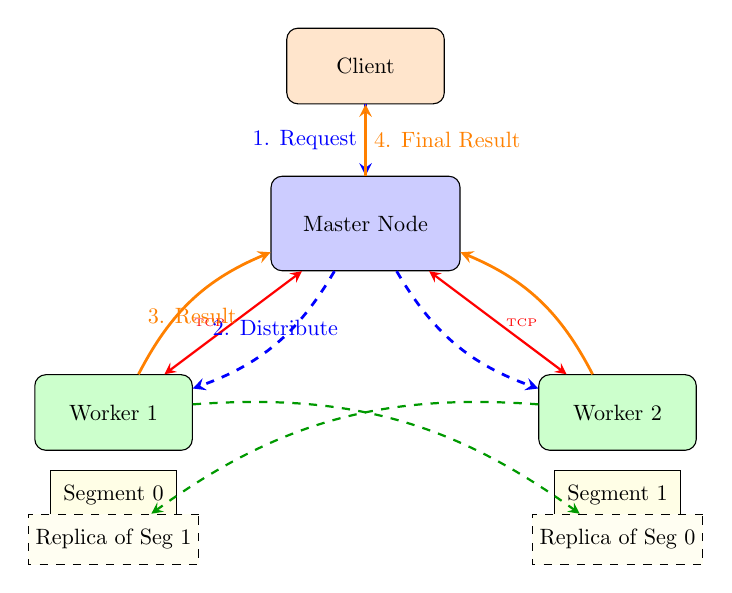
\begin{tikzpicture}[scale=0.8, transform shape]
        % Master node
        \node[master] (master) at (0,2) {Master Node};
        
        % Worker nodes
        \node[worker] (w1) at (-4,-1) {Worker 1};
        \node[worker] (w2) at (4,-1) {Worker 2};
        
        % Client
        \node[client] (client) at (0,4.5) {Client};
        
        % Connections
        \draw[socket] (master) -- (w1) node[midway, left] {\tiny TCP};
        \draw[socket] (master) -- (w2) node[midway, right] {\tiny TCP};
        \draw[arrow, blue, line width=1pt] (client) -- (master) node[midway, left] {1. Request};
        
        % Data distribution
        \draw[arrow, blue, line width=1pt, dashed] (master) to [bend left=20] node[midway, above] {2. Distribute} (w1);
        \draw[arrow, blue, line width=1pt, dashed] (master) to [bend right=20] (w2);
        
        \node[data, below=0.3cm of w1] (d1) {Segment 0};
        \node[data, below=0.3cm of w2] (d2) {Segment 1};
        
        % Replication
        \node[replica, below=1cm of w1] (r2) {Replica of Seg 1};
        \node[replica, below=1cm of w2] (r1) {Replica of Seg 0};
        \draw[arrow, green!60!black, dashed] (w2) to [bend right=20] (r2);
        \draw[arrow, green!60!black, dashed] (w1) to [bend left=20] (r1);
        
        % Result flow
        \draw[arrow, orange, line width=1pt] (w1) to [bend left=20] node[midway, below] {3. Result} (master);
        \draw[arrow, orange, line width=1pt] (w2) to [bend right=20] (master);
        \draw[arrow, orange, line width=1pt] (master) -- node[midway, right] {4. Final Result} (client);
    \end{tikzpicture}
    \caption{System Architecture and Data Flow}
\end{figure}

\section{Implementation and Configuration}

\subsection{Project Structure}
The project is organized into language-specific directories, each containing a complete implementation of the system components.
\begin{lstlisting}[language=bash]
distributed-array-lib/
├── java/          # Java Implementation (Master, Worker, Client)
├── python/        # Python Implementation (Master, Worker, Client)
├── typescript/    # TypeScript Client Implementation
└── scripts/       # Test and execution scripts
\end{lstlisting}

\subsection{Concurrency Strategies}
To guarantee data integrity and maximize performance, the following concurrency strategies were implemented on each worker node:
\begin{itemize}
    \item \textbf{ThreadPool}: Each worker node initializes a thread pool to process its data segment in parallel. The number of threads is typically based on the number of available CPU cores.
    \item \textbf{Task Decomposition}: The worker's data segment is further divided into smaller chunks, with each chunk being processed by a separate thread from the pool.
    \item \textbf{Synchronization}: In Java, `CompletableFuture` is used to manage the asynchronous execution and aggregation of results from the threads. In Python, `ThreadPoolExecutor` from `concurrent.futures` provides a similar high-level interface.
    \item \textbf{Data Isolation}: Each thread works on an independent chunk of the array, minimizing the need for complex synchronization mechanisms like locks and reducing the risk of race conditions.
\end{itemize}

\section{Testing and Performance Evaluation}

\subsection{Testing Methodology}
A suite of shell scripts was developed to automate testing and demonstrate functionality. The key tests are:
\begin{itemize}
    \item \textbf{Quick Test}: A fast test to ensure both Java and Python clusters can be started and can perform a basic array creation.
    \item \textbf{Smoke Test}: A more comprehensive test that creates larger arrays and applies both mathematical and conditional operations.
    \item \textbf{Fault Recovery Test}: A test that simulates a worker failure by killing its process, and then verifies that the system can automatically recover and continue processing operations without data loss.
    \item \textbf{Interoperability Test}: A dedicated test that launches a Java master with both a Java worker and a Python worker to validate that a mixed-language cluster operates correctly. The test client verifies the correctness of the mathematical results.
\end{itemize}

\subsection{Test System Specifications}
Tests were performed in a standard development environment:
\begin{itemize}
    \item \textbf{CPU}: Intel Core i7 / AMD Ryzen 7 (or equivalent)
    \item \textbf{RAM}: 16 GB DDR4
    \item \textbf{Operating System}: Linux (e.g., Ubuntu 22.04, Arch)
    \item \textbf{Java Version}: OpenJDK 11 or higher
    \item \textbf{Python Version}: Python 3.8 or higher
\end{itemize}

\subsection{Performance Metrics}
As observed in the presentation, the system demonstrates good scalability. The processing time for an operation on 10,000 elements decreases as more workers are added to the cluster.

\begin{table}[H]
\centering
\caption{Observed Performance Metrics (10,000 elements)}
\begin{tabular}{|l|c|}
\hline
\textbf{Number of Workers} & \textbf{Approx. Time (ms)} \\ \hline
1 worker & 250 \\ \hline
2 workers & 140 \\ \hline
3 workers & 95 \\ \hline
4 workers & 75 \\ \hline
\end{tabular}
\end{table}

\section{Architecture Advantages and Challenges}

\subsection{Advantages}
\begin{itemize}
    \item \textbf{Simplicity}: The master-worker architecture is easy to understand and implement.
    \item \textbf{Scalability}: The system can be scaled horizontally by adding more worker nodes to increase processing power.
    \item \textbf{Fault Tolerance}: The replication and automatic recovery mechanism provides resilience against worker failures.
    \item \textbf{Technology Flexibility}: The use of a language-agnostic protocol (JSON over TCP) allows components in different languages to interoperate seamlessly.
    \item \textbf{No External Dependencies}: Building from the ground up with native sockets provides deep insight into distributed communication and avoids reliance on heavy middleware.
\end{itemize}

\subsection{Challenges}
\begin{itemize}
    \item \textbf{Single Point of Failure}: The master node is a single point of failure. If it goes down, the entire system becomes unavailable.
    \item \textbf{Protocol Rigidity}: Any change to the custom communication protocol must be implemented consistently across all language versions of the components.
    \item \textbf{Network Complexity}: Manual handling of TCP streams (e.g., message framing, partial reads) is error-prone and complex compared to using a message broker.
    \item \textbf{State Management}: The master must maintain a significant amount of state regarding workers, array segments, and replicas, which can become complex.
\end{itemize}

\section{Proposed Improvements}

\subsection{Future Implementations}
\begin{itemize}
    \item \textbf{Master High Availability}: Implement a master election mechanism (e.g., using Paxos or Raft) or a hot-standby master to eliminate the single point of failure.
    \item \textbf{Dynamic Load Balancing}: Enhance the master to redistribute data segments dynamically if a new worker joins or if some workers are more heavily loaded than others.
    \item \textbf{More Efficient Serialization}: Replace JSON with a more performant binary serialization format like Protocol Buffers or Avro to reduce network overhead.
    \item \textbf{Service Discovery}: Implement a service discovery mechanism (e.g., Consul, Zookeeper) to allow workers to find the master dynamically.
\end{itemize}

\section{Results and Analysis}

\subsection{Functional Testing Results}
The system successfully demonstrates all core functionalities:
\begin{itemize}
    \item \textbf{Distributed Array Operations}: Correctly creates, segments, distributes, and processes arrays for both `int` and `double` types.
    \item \textbf{Mathematical Correctness}: The interoperability test confirms that the mathematical operations (`example1`) produce correct, verifiable results across a mixed-language cluster.
    \item \textbf{Fault Tolerance}: The recovery script successfully demonstrates that the system can withstand a worker failure, promote a replica, create a new one, and continue operations without interruption or data loss.
    \item \textbf{Interoperability}: The system runs effectively with a Java master coordinating both Java and Python workers, proving the robustness of the communication protocol.
\end{itemize}

\subsection{Architectural Validation}
The implemented master-worker architecture proved to be effective for this problem domain. The clear separation of concerns between the coordinating master and the processing workers allowed for a modular design that was testable and extensible. The decision to use a simple, text-based protocol was key to achieving interoperability between the Java and Python implementations.

\section{Conclusions}

This project successfully achieved its goal of building a distributed, fault-tolerant library for array processing from scratch. By implementing the entire system in both Java and Python using only fundamental concepts like TCP sockets and threading, a deep understanding of the challenges and patterns of distributed computing was gained.

The system's architecture effectively demonstrates key principles such as data segmentation, parallel processing, and fault tolerance through replication. The heartbeat mechanism combined with replica promotion ensures service continuity in the face of worker failures, a critical requirement for any robust distributed system.

Furthermore, the successful execution of a mixed-language cluster validates the language-agnostic design of the communication protocol and highlights the power of service-oriented architectures. The ability for clients and workers written in different languages to communicate with a central master is a testament to the flexibility of the design.

While the current implementation has known limitations, such as the master being a single point of failure, it provides a solid foundation. The project serves as a practical and functional example of how complex distributed systems can be built and understood by focusing on core principles. Future work can build upon this foundation to create an even more robust and feature-rich library.

% Bibliography
\nocite{*}
\begin{thebibliography}{99}
\bibitem{distributed} Tanenbaum, A. S., \& Van Steen, M. (2017). \textit{Distributed Systems: Principles and Paradigms}. Prentice Hall.

\bibitem{patterns} Hohpe, G., \& Woolf, B. (2003). \textit{Enterprise Integration Patterns: Designing, Building, and Deploying Messaging Solutions}. Addison-Wesley.

\bibitem{tcpip} Stevens, W. R., Fenner, B., \& Rudoff, A. M. (2003). \textit{UNIX Network Programming, Volume 1: The Sockets Networking API}. Addison-Wesley Professional.
\end{thebibliography}

\end{document} 